\documentclass[11pt]{article}
\oddsidemargin=17pt \evensidemargin=17pt
\headheight=9pt     \topmargin=26pt
\textheight=564pt   \textwidth=433.8pt

\usepackage{url}
\usepackage{amsmath}
\usepackage{amsfonts,amssymb,amsthm,cite,float,graphicx}
\usepackage{physics}
\usepackage{graphicx}
\usepackage{mathtools}
\usepackage{float}

%new math symbols taking no arguments
\newcommand\0{\mathbf{0}}
\newcommand\CC{\mathbb{C}}
\newcommand\FF{\mathbb{F}}
\newcommand\NN{\mathbb{N}}
\newcommand\QQ{\mathbb{Q}}
\newcommand\RR{\mathbb{R}}
\newcommand\ZZ{\mathbb{Z}}
\newcommand\bb{\mathbf{b}}
\newcommand\kk{\Bbbk}
\newcommand\mm{\mathfrak{m}}
\newcommand\pp{\mathfrak{p}}
\newcommand\xx{\mathbf{x}}
\newcommand\yy{\mathbf{y}}
\newcommand\GL{\mathit{GL}}
\newcommand\into{\hookrightarrow}
\newcommand\nsub{\trianglelefteq}
\newcommand\onto{\twoheadrightarrow}
\newcommand\minus{\smallsetminus}
\newcommand\goesto{\rightsquigarrow}
\newcommand\nsubneq{\vartriangleleft}

%redefined math symbols taking no arguments
\newcommand\<{\langle}
\renewcommand\>{\rangle}
\renewcommand\iff{\Leftrightarrow}
\renewcommand\phi{\varphi}
\renewcommand\implies{\Rightarrow}

%new math symbols taking arguments
\newcommand\ol[1]{{\overline{#1}}}

%redefined math symbols taking arguments
\renewcommand\mod[1]{\ (\mathrm{mod}\ #1)}

%roman font math operators
\DeclareMathOperator\aut{Aut}

%for easy 2 x 2 matrices
\newcommand\twobytwo[1]{\left[\begin{array}{@{}cc@{}}#1\end{array}\right]}

%for easy column vectors of size 2
\newcommand\tworow[1]{\left[\begin{array}{@{}c@{}}#1\end{array}\right]}

\newtheorem{theorem}{Theorem}[section]
\newtheorem{corollary}{Corollary}[theorem]
\newtheorem{lemma}[theorem]{Lemma}
\newtheorem{exercise}[theorem]{Exercise}

\title{Quantum Algorithms and Learning Theory\\\textit{Notes and Exercises}}
\author{Faris Sbahi}

\begin{document}
\maketitle

\section{Nielsen \& Chuang: Chapter 2}

\subsection{Postulates of Quantum Mechanics}

First, we cover the fundamental postulates of quantum mechanics. 

\subsubsection{State Space and State Vector}

Associated with an isolated physical system is a Hilbert space, $\mathcal{H}$. A Hilbert space is a complete inner-product vector space. Note that completeness holds trivially in a finite-dimensional vector space because we have closure with respect to all sequences (and hence any Cauchy sequence in the vector space must converge to a vector in the same space). Nevertheless, the state space of a physical system may be infinite-dimensional. 

A system is completely described by a unit vector $u \in \mathcal{H}$ called the state vector.

For example, consider a system given by a single qubit, which has a two-dimensional state space. Let $\ket{0}$ and $\ket{1}$ be an orthonormal basis for this space. Hence, a state vector in this space is given by 

\begin{align*}
\ket{\psi} = a\ket{0} + b\ket{1}	
\end{align*}


where $a, b \in \CC$ and $|a|^2 + |b|^2 = 1$. 

\subsubsection{Evolution}\label{post-discrete-evol}

The evolution of a closed quantum system is described by a unitary transformation. Recall that an operator $U$ is unitary iff $U^\dagger U = I = UU^\dagger$ (and hence preserves inner products\footnote{and furthermore has a spectral decomposition because it is normal}).

So, let the state of a system at time $t_1$ be given by $\ket{\psi}$ and $\ket{\psi'}$ at $t_2$. Hence,

\begin{align*}
\ket{\psi'} = U\ket{\psi}	
\end{align*}

\subsubsection{Evolution in Continuous Time}\label{post-cts-evol}

Schrodinger's equation provides the time evolution of the state of a quantum system

\begin{align}\label{schro-cts}
i\hbar \frac{d\ket{\psi}}{dt} = H\ket{\psi}	
\end{align}

where $H$ is the (Hermitian) Hamiltonian of the closed system. Because the Hamiltonian is Hermitian it has spectral decomposition 

\begin{align*}
H = \sum_{E} E \ket{E}\bra{E}	
\end{align*}

where $E$ is the energy eigenvalue corresponding to energy eigenstate $\ket{E}$. 

For example, consider the Hamiltonian $H = \hbar \omega X$  (recall that $X = \sigma_X = \begin{pmatrix} 0 & 1 \\ 1 & 0\end{pmatrix}$ from \ref{pauli}). Hence, we solve for its eigenvalues and eigenvectors

\begin{align*}
	\det{ \hbar\omega\begin{pmatrix} -\lambda & 1 \\ 1 & -\lambda\end{pmatrix}} &= 0 \\
	\lambda^2 - 1^2 &= 0 \\
	\lambda &= \pm 1 \\
	\implies E_{\pm} &= \pm \hbar \omega \\
	\hbar\omega\begin{pmatrix} -1 & 1 \\ 1 & -1\end{pmatrix}\ket{E_+} &= 0 \\
	\ket{E_+} &= \frac{1}{\sqrt{2}}\begin{pmatrix}
		1 \\ 1
	\end{pmatrix} \coloneqq \ket{+} \\
	\ket{E_-} &= \ket{-}
\end{align*}

Onwards, notice that we can solve Schrodinger's equation (\ref{schro-cts}) and have

\begin{align*}
	\ket{\psi(t_2)} &= \exp[\frac{-iH(t_2 - t_1)}{\hbar}] \ket{\psi(t_1)}
\end{align*}

and equivalently from \ref{post-discrete-evol} we can represent this transformation with unitary operator $U = \exp[\frac{-iH(t_2 - t_1)}{\hbar}]$. This holds in general and so we can consider the two descriptions from \ref{post-discrete-evol} and \ref{post-cts-evol} interchangeably (the authors prefer the latter). 

\subsubsection{Quantum Measurement}\label{qmeas}

Quantum measurements are described by a collection of measurements operators $\{ M_m \}$ (where the index $m$ refers to the potential measurement outcomes of the experiment) which act on the state space of the system being observed. 

Hence, if the pre-measurement state is $\ket{\psi}$, then 

\begin{align*}
	p(m) = \bra{\psi} M_m^\dagger M_m \ket{\psi}
\end{align*}

and the post-measurement state is 

\begin{align*}
	\frac{M_m \ket{\psi}}{\sqrt{p(m)}}
\end{align*}

Furthermore, $\{ M_m \}$ satisfy the completeness equation

\begin{align*}
\sum_m M_m^\dagger M_m = I
\end{align*}

An important example of a measurement is the measurement of a qubit in the computational basis. This is a measurement of a qubit with two outcomes defined by the measurement operators $M_0 = \ket{0}\bra{0}$ and $M_1 = \ket{1}\bra{1}$.

Now, we see an interesting implication. If we seek to distinguish our physical system from a set of orthogonal states, then we can reliably do so by simply defining each measurement operator to be the outer product of our states of interest. We add a final operator defined to be the remaining complement of the identity in order to satisfy the completeness equation. 

On the flipside, two non-orthogonal states $\ket{\psi_1}$ and $\ket{\psi_2}$ necessarily share a parallel component in their orthogonal decomposition. Hence, a measurement outcome that corresponds to the pre-measurement state being $\ket{\psi_1}$ with probability $p > 0$ has a probability $p'>0$ of having been in state $\ket{\psi_2}$. 

\subsubsection{Projective Measurements}

There exists a special class of quantum measurements known as projective measurements. These measurements can be described by an observable $M$, a hermitian operator on the state space being observed. $M$ has spectral decomposition

\begin{align*}
M = \sum_m m P_m	
\end{align*}

where $P_m$ is the projector onto the eigenspace of $M$ with eigenvalues $m$. 

Furthermore, if the pre-measurement state is $\ket{\psi}$, then 

\begin{align*}
p(m) = 	\bra{\psi} P_m \ket{\psi}
\end{align*}

and the post-measurement state is 

\begin{align*}
	\frac{P_m \ket{\psi}}{\sqrt{p(m)}}
\end{align*}

This simplifies the formula for the expected value of a measurement

\begin{align*}
\langle M \rangle &= \sum_m m p(m) \\
&= \bra{\psi} (\sum_m m P_m)  \ket{\psi} \\
&= 	\bra{\psi} M \ket{\psi}
\end{align*}

For example, consider projective measurements on the system given by single qubits with observable Pauli matrix $Z$. Hence, $Z$ has eigenvalues $+1$ and $-1$ and eigenstates $\ket{0}$ and $\ket{1}$, respectively. So, consider state $\ket{\psi} = \frac{\ket{0} + \ket{1}}{\sqrt{2}}= \ket{+}$ $\implies$ $p(+1) = \bra{+}\ket{0}\bra{0}\ket{+} = \frac{1}{2}$. Similarly, $p(-1) = \frac{1}{2}$. 

More generally, suppose $v$ is an arbitrary 3-d vector. We can define an observable

\begin{align*}
v \cdot \sigma = v_1\sigma_x + v_2 \sigma_y + v_3\sigma_z
\end{align*} 

\subsubsection{POVM measurements}\label{povm}

POVMs are best viewed as a special case of the general measurement formalism, providing the simplest means to study post-measurement statistics without knowledge of the post measurement state.

From above, $p(m) = \bra{\psi} M_m^\dagger M_m \ket{\psi}$ so if we define $E_m \coloneqq M_m^\dagger M_m$ (which is hence positive from \ref{posop}) then these $E_m$'s are sufficient for the purpose of computing probabilities. We denote $\{ E_m \}$ as a POVM. 

Note that projective operators are the special case of being equivalent to their respective POVM element because $E_m = P_m^\dag P_m = P_m$. 

Nevertheless, the POVM formalism is a useful guide in for our intuition in quantum information. Consider if Alice prepares some state for Bob that is either $\ket{\psi_1} = \ket{0}$ or $\ket{\psi_2} = \frac{\ket{0} + \ket{1}}{\sqrt{2}}$. Recall from \ref{qmeas}, Bob can't determine which state was prepared with full certainty (because of the shared orthogonal component $\ket{0}$). Still, we can define a POVM\footnote{verify that completeness and these being positive operators holds}

\begin{align*}
E_1 &= \frac{\sqrt{2}}{1+\sqrt{2}}\ket{1}\bra{1}	\\
E_2 &= \frac{\sqrt{2}}{1+\sqrt{2}}\frac{(\ket{0} - \ket{1})(\bra{0} - \bra{1})}{2} \\
E_3 &= I - E_1 - E_2
\end{align*}

Now, notice what happens. 

\begin{align*}
\bra{\psi_1} E_1 \ket{\psi_1} &= \bra{0} \frac{\sqrt{2}}{1+\sqrt{2}}\ket{1}\bra{1}\ket{0} \\
	&= 0 \\
\bra{\psi_2} E_1 \ket{\psi_2} &= \frac{\bra{0} + \bra{1}}{\sqrt{2}}\frac{\sqrt{2}}{1+\sqrt{2}}\ket{1}\bra{1}\frac{\ket{0} + \ket{1}}{\sqrt{2}} \\
	&= \frac{\sqrt{2}}{2\sqrt{2} + 2} > 0 
\end{align*}

Hence, if we observe $E_1$ after the measurement described by $\{ E_1, E_2, E_3 \}$, then Alice must've prepared $\ket{\psi_2}$. Similarly,

\begin{align*}
\bra{\psi_1} E_2 \ket{\psi_1} &= \bra{0} \frac{\sqrt{2}}{1+\sqrt{2}}\frac{(\ket{0} - \ket{1})(\bra{0} - \bra{1})}{2}\ket{0} \\
	&= \frac{\sqrt{2}}{2\sqrt{2} + 2} > 0 \\
\bra{\psi_2} E_2 \ket{\psi_2} &= \frac{\bra{0} + \bra{1}}{\sqrt{2}}\frac{\sqrt{2}}{1+\sqrt{2}}\frac{(\ket{0} - \ket{1})(\bra{0} - \bra{1})}{2}\frac{\ket{0} + \ket{1}}{\sqrt{2}} \\
	&= 0
\end{align*}

so if we observe $E_2$, then Bob concludes that Alice prepared $\ket{\psi_1}$. Our routine is imperfect because we may observe $E_3$ and hence would infer nothing of the original state. Still, we would never $\textit{incorrectly}$ guess given that we allow ourselves to abstain when we see $E_3$. 

\begin{exercise} (2.64) Suppose Bob is given a quantum state chosen from a set $S = \ket{\psi_1} , \cdots , \ket{\psi_m}$ of linearly independent states. Construct a POVM $\{ E_1 , \cdots , E_{m+1} \}$ such that if outcome $E_i$ occurs, $1 \leq i \leq m$, then Bob knows with certainty that he was given state $\ket{\psi_i}$.
\end{exercise}

To distinguish the states we require $\bra{\psi_i} E_j \ket{\psi_i} = p_i \delta_{ij}$ where $p_i > 0$ and $1 \leq i,j \leq m$. 

So, we can use the Gram-Schmidt process using $S$ as our linearly independent set. This will give us an orthonormal set $U = \ket{\phi_1} , \cdots , \ket{\phi_m}$ that spans the same subspace as $S$. Next, we can represent each $\ket{\psi_i}$ in this orthonormal basis, $U$. Finally, for each $i$ we can find a vector $\ket{\psi'_i}$ in the span of $U$ that is orthogonal to all $\ket{\psi_j}, j \neq i$. Hence, we can define $E_i = \ket{\psi_i'} \bra{\psi_i'}, 1 \leq i \leq m$. Finally, take $E_{m+1} = I - \sum_m E_i$. 

Creating an optimal POVM is much trickier (in the sense of minimizing the probability $p_{m+1}$).

From this exercise, we see that POVMs present a reliable way to distinguish non-orthogonal (but linearly independent) states given that we allow for the slack of an "inconclusive" measurement ($E_{m+1}$). 

\subsubsection{Composite Systems}

The state space of a composite physical system is the tensor product of the state spaces of the component physical systems. 

\begin{exercise} (2.66)
	Show that the average value of the observable $X_1Z_2$ ($X$ acting on the first qubit and $Z$ on the second) for a two qubit system measured in the state $\frac{\ket{00} + \ket{11}}{\sqrt{2}}$ is zero.
\end{exercise}

\begin{proof}
	Let observable $M = X_1Z_2$. Hence, 
	
	\begin{align*}
	\langle M \rangle &= \frac{\bra{00} + \bra{11}}{\sqrt{2}} M \frac{\ket{00} + \ket{11}}{\sqrt{2}}\\	
	&= \frac{\bra{00} + \bra{11}}{\sqrt{2}}\frac{X_1\ket{0}Z_2\ket{0} + X_1\ket{1}Z_2\ket{1}}{\sqrt{2}} \\
	&= \frac{\bra{00} + \bra{11}}{\sqrt{2}}\frac{\ket{1}\ket{0} - \ket{0}\ket{1}}{\sqrt{2}} \\
	&= 0
	\end{align*}
\end{proof}
 
Interestingly, we can show that a general quantum measurement (as described in \ref{qmeas}) can be implemented as a projective measurement coupled with unitary dynamics.

Consider a quantum system with state space $Q$ and measurements $M_m$ on this system. We can introduce an \textit{ancilla} system $M$ with orthonormal basis $\ket{m}$ which is in one-to-one correspondence with the possible outcomes of the measurement we wish to implement. 

So, let $\ket{0}$ be a fixed state of $M$ and define an operator $U$ on $\ket{\psi}\ket{0}$ (with $\ket{\psi}$ as a state of $Q$) by

\begin{align*}
U\ket{\psi}\ket{0} \coloneqq \sum_m M_m \ket{\psi}\ket{m}
\end{align*}

Hence,

\begin{align*}
\bra{\phi}\bra{0}U^\dag U \ket{\psi}	 \ket{0} &= \sum_m \sum_{m'} \bra{\phi} M_m^\dag M_{m'} \ket{\psi}\bra{m}\ket{m'} \\
\intertext{So, because the states $\ket{m}$ are orthonormal}
&= \sum_m\bra{\phi} M_m^\dag M_{m} \ket{\psi} \\
\intertext{and finally by the completeness of $M_m$}
&= \bra{\phi}\ket{\psi}
\end{align*}

This tells us that $U$ preserves inner products between states of the form $\ket{\psi}\ket{0}$. Furthermore, we can show that $U$ can be extended to a unitary operator on $Q \otimes M$ (exercise).

Hence, consider a projective measurement on the two systems ($U\ket{\psi}\ket{0}$) given by projectors $P_m \coloneqq I_Q \otimes \ket{m}\bra{m}$. So,

\begin{align*}
p(m) &= \bra{\psi} \bra{0} U^\dag P_m U \ket{\psi} \ket{0} \\
&= \sum_{m'}\sum_{m''} \bra{\psi} M_{m'}^\dag \bra{m'} (I_Q \otimes \ket{m}\bra{m})M_{m''} \ket{\psi} \ket{m''} \\
&= \bra{\psi} M_m^\dag M_m \ket{\psi}
\end{align*}

which agrees with the general result from \ref{qmeas}. Similarly, the post-measurement state is as expected. Hence, we've shown that unitary dynamics, projective measurements, and ancillary systems can be used together to describe any general measurement.

\begin{exercise}
(2.68) Prove that $\ket{\psi} \neq \ket{a}\ket{b}$ for all single qubit state $\ket{a}$ and $\ket{b}$ where $\ket{\psi} = \frac{\ket{00} + \ket{11}}{\sqrt{2}}$.
\end{exercise}

\begin{proof}
	First, decompose the qubit state in their basis, $\ket{a} = \alpha_0 \ket{0} + \alpha_1 \ket{1}$ and $\ket{b} = \beta_0 \ket{0} + \beta_1 \ket{1}$. Now, we prove by contradiction
	
	\begin{align*}
	\ket{a}\ket{b} &= \alpha_0\beta_0 \ket{00} + \alpha_0\beta_1 \ket{01} + \alpha_1\beta_0 \ket{10} + \alpha_1\beta_1 \ket{11} \\
	&= \frac{\ket{00} + \ket{11}}{\sqrt{2}}
	\end{align*}

which would imply that either $\alpha_0$ or $\beta_1$ are zero in order to remove the $\ket{01}$ term. However, this would also remove either the $\ket{00}$ or $\ket{11}$ term, so we have a contradiction.
\end{proof}

A state of a composite system having this property is said to be entangled. 

\subsection{Superdense Coding}

Suppose Alice is in possession of two classical bits of information she wishes to transmit to Bob, but is only allowed to send a single qubit to Bob.

 Now, suppose that Alice and Bob initially share a pair of qubits in the entangled state from above
 
\begin{align*}
\ket{\psi} = \frac{\ket{00} + \ket{11}}{\sqrt{2}}	
\end{align*}
 
 where Alice is initially holding the first qubit and Bob the second. She can then apply a particular gate to send a bit string. Below shows the corresponding gate and resulting state
 
 \begin{table}[H]
 	\begin{center}
 \begin{tabular}{l | c | l }
 	Bit String & Applied gate  & Resulting state\\
 	\hline 
 	00 & -- & $\frac{\ket{00} + \ket{11}}{\sqrt{2}}$\\
 	01 & Z & $\frac{\ket{00} - \ket{11}}{\sqrt{2}}$\\
 	10 & X & $\frac{\ket{10} + \ket{01}}{\sqrt{2}}$\\
 	11 & iY & $\frac{-\ket{10} + \ket{01}}{\sqrt{2}}$
 \end{tabular}
 \end{center}
 \end{table}

Observe that these are the Bell states (see \ref{bellstates}). Furthermore, Bell states form an orthonormal basis and hence can be distinguished (as we've discussed in \ref{povm}). Hence, Alice needs only to interact with the single qubit to transmit two classical bits of information to Bob.

\begin{exercise} 
(2.70) Suppose $E$ is any positive operator acting on Alice’s qubit. Show that $\bra{\psi} E \otimes I \ket{\psi}$ takes the same value when $\ket{\psi}$ is any of the four Bell states. Suppose some malevolent third party ('Eve') intercepts Alice’s qubit on the way to Bob in the superdense coding protocol. Can Eve infer anything about which of the four possible bit strings 00, 01, 10, 11 Alice is trying to send? If so, how, or if not, why not?	
\end{exercise}

\begin{proof}
\begin{align*}
	\bra{00} + \bra{11} (E \otimes I) \ket{00} + \ket{11} &= \bra{0}E\ket{0} + \bra{1}E\ket{1}\\
 	\bra{00} - \bra{11}(E \otimes I)\ket{00} - \ket{11}&= \bra{0}E\ket{0} + \bra{1}E\ket{1}\\
 	\bra{10} + \bra{01} (E \otimes I)\ket{10} + \ket{01} &= \bra{0}E\ket{0} + \bra{1}E\ket{1}\\
 	-\bra{10} + \bra{01}(E \otimes I)-\ket{10} + \ket{01} &= \bra{0}E\ket{0} + \bra{1}E\ket{1}\\
\end{align*}
	
	Hence, Eve can't infer anything. The states are only distinguishable if one can perform a measurement that acts on both qubits.  
\end{proof}


\subsection{The Density Operator}

An alternative formulation of quantum mechanics is possible using a tool known as the density operator. 

Suppose a quantum system is one of a number of states $\ket{\psi}$ with probability $p_i$. We call $\{p_i, \ket{\psi_i} \}$ an ensemble of pure states. The density operator is defined

\begin{align*}
\rho \coloneqq \sum_i p_i \ket{\psi_i}\bra{\psi_i}	
\end{align*}

Evolution of the density operator (under a unitary transformation) can be derived readily

\begin{align*}
\sum_i p_i U\ket{\psi_i}\bra{\psi_i}U^\dag = U\rho U^\dag	
\end{align*}

If we perform a measurement with operator $M_m$ with initial state $\ket{\psi_i}$ then

\begin{align*}
p(m\mid i) &= \bra{\psi_i} M_m^\dag M_m \ket{\psi_i} \\
&= \tr(M_m^\dag M_m \ket{\psi_i}\bra{\psi_i})
\end{align*}

using \ref{trop}. 

Hence, summing this conditional probability across all initial states we have

\begin{align*}
	p(m) &= \sum_i p_i \tr(M_m^\dag M_m \ket{\psi_i}\bra{\psi_i}) \\
	&= \tr(M_m^\dag M_m \rho)
\end{align*}

The state after obtaining measurement result $m$ on initial state $\ket{\psi_i}$ is

\begin{align*}
\ket{\psi_i^m} = \frac{M_m \ket{\psi_i}}{\sqrt{\bra{\psi_i}M_m^\dag M_m\ket{\psi_i}}}	
\end{align*}

and so the density operator after result $m$ is given by

\begin{align*}
	\rho_m &= \sum_i p(i \mid m ) \ket{\psi_i^m} \bra{\psi_i^m} \\
	&= \sum_i p(i \mid m )\frac{M_m \ket{\psi_i}\bra{\psi_i}M_m^\dag}{\bra{\psi_i}M_m^\dag M_m\ket{\psi_i}}
\end{align*}

Furthermore, from Baye's rule we have that $p(i \mid m) = \frac{p(m \mid i)p(i)}{p(m)}$ so we can simplify

\begin{align*}
	\rho_m &= \sum_i \frac{p(m \mid i)p(i)}{p(m)}\frac{M_m \ket{\psi_i}\bra{\psi_i}M_m^\dag}{\bra{\psi_i}M_m^\dag M_m\ket{\psi_i}} \\
	&= \sum_i \frac{p(i)\bra{\psi_i} M_m^\dag M_m \ket{\psi_i}}{\tr(M_m^\dag M_m \rho)}\frac{M_m \ket{\psi_i}\bra{\psi_i}M_m^\dag}{\bra{\psi_i}M_m^\dag M_m\ket{\psi_i}} \\
	&= \sum_i \frac{p(i)M_m \ket{\psi_i}\bra{\psi_i}M_m^\dag}{\tr(M_m^\dag M_m \rho)} \\
	&= \frac{M_m\rho M_m^\dag}{\tr(M_m^\dag M_m \rho)}
\end{align*}

A quantum state whose state $\ket{\psi}$ is known exactly is said to be in a pure state. In this case the density operator is simply $\rho = \ket{\psi}\bra{\psi}$. Otherwise, $\rho$ is in a mixed state.

A pure state satisfies $\tr(\rho^2) = 1$ and a mixed state $\tr(\rho^2) < 1$.

Imagine that our record of the result $m$ of a measurement was lost. We would have a quantum system in the state $\rho_m$ with probability $p(m)$ without knowing the actual value of $m$. Hence, the system would be described as

\begin{align*}
\rho &= \sum_m p(m) \rho_m	\\
&= \sum_m M_m \rho M_m^\dag 
\end{align*}

We may wish to move away from the interpretation of the density operator as a means of describing ensembles of quantum states.

\begin{theorem}
An operator $\rho$ is a density operator associated to some ensemble $\{p_i, \ket{\psi_i}\}$ if and only if it satisfies the conditions

\begin{enumerate}
\item $\rho$ has trace equal to one
\item $\rho$ is a positive operator	
\end{enumerate}

\begin{proof}
	We show one direction (see the text for the other). Let $\rho$ be a density operator. Hence,
	
	\begin{align*}
	\tr(\rho) &= \sum_i p_i \tr(\ket{\psi_i}\bra{\psi_i}) \\
	&= 	\sum_i p_i =1
	\end{align*}

because $\tr(\ket{\psi_i}\bra{\psi_i}) = \psi_{i1}^2 + \psi_{i2}^2 + \cdots \psi_{in}^2 = 1$ by normalization. 

Furthermore, suppose $\ket{\phi}$ resides in the vector space

\begin{align*}
\bra{\phi} \rho \ket{\phi} &= \sum_i p_i \bra{\phi}\ket{\psi_i}\bra{\psi_i}\ket{\phi} \\
&= \sum_i p_i |\bra{\phi}\ket{\psi_i}|^2 \geq 0
\end{align*}
so we have positivity.
\end{proof}	
\end{theorem}

The use of this theorem is that we can define a density operator to be a positive operator with trace one and hence reformulate the postulates of quantum mechanics without speaking of ensembles.

This reformulation shines when describing quantum systems whose state is not known and when describing subsystems a composite quantum system.

\begin{exercise}
(2.71) Let $\rho$ be a density operator. Show that $\tr(\rho^2) \leq 1$ with equality iff $\rho$ is a pure state.
\begin{proof}
% TODO (2.71)	
\end{proof}	
\end{exercise}

Remember that different ensembles of quantum states can give rise to a specific density matrix and hence one must avoid assuming that the eigenvectors and eigenvalues have special significance with regard to the represented ensemble of quantum states.

Nevertheless, there is value in discussing which ensembles give rise to the same density matrix (notably in quantum noise and error correction). Let $\ket{\tilde{\psi_i}}$ generate $\rho$ i.e. $\rho\coloneqq\sum_i\ket{\tilde{\psi_i}}\bra{\tilde{\psi_i}}$. Note that $\ket{\tilde{\psi_i}} = \sqrt{p_i}\ket{\psi_i}$ is clearly not necessarily normalized. Now, we have the following theorem.

\begin{theorem}
The sets $\ket{\tilde{\psi_i}}$ and $\ket{\tilde{\phi_j}}$ generate the same $\rho$ if and only if

\begin{align*}
	\ket{\tilde{\psi_i}} = \sum_j u_{ij}\ket{\tilde{\phi_j}}
\end{align*}

where the matrix with matrix elements $u_{ij}$ is unitary.
\begin{proof}
	See the text.
\end{proof}
\end{theorem}

\begin{exercise}
(2.72) Bloch Sphere for mixed states.
\begin{proof}
% TODO (2.72)	
\end{proof}	
\end{exercise}

As mentioned above, density operators are powerful tools for describing subsystems of composite systems. 
 
Suppose we have physical systems $A$ and $B$, whose state is described by $\rho^{AB}$. The reduced density operator for system $A$ is defined by

\begin{align*}
\rho^A \coloneqq \tr_B(\rho^{AB})
\end{align*}

where $\tr_B$ is a map of operators known as the partial trace over system $B$ which is defined by

\begin{align*}
\tr_B(\ket{a_1}\bra{a_2} \otimes \ket{b_1}\bra{b_2}) &= \ket{a_1}\bra{a_2} \tr( \ket{b_1}\bra{b_2}) \\
&= \ket{a_1}\bra{a_2} \bra{b_2}\ket{b_1}
\end{align*}

Hence, consider the Bell state $\frac{\ket{00} + \ket{11}}{\sqrt{2}}$ and the reduced density operator of its first qubit

\begin{align*}
\rho &= \frac{\ket{00} + \ket{11}}{\sqrt{2}}\frac{\bra{00} + \bra{11}}{\sqrt{2}} \\
\rho^1 &= \frac{\ket{0}\bra{0}\bra{0}\ket{0}+\ket{1}\bra{0}\bra{0}\ket{1}+ \ket{0}\bra{1}\bra{1}\ket{0}+ \ket{1}\bra{1}\bra{1}\ket{1}}{2} \\
&= \frac{\ket{0}\bra{0} + \ket{1}\bra{1}}{2} \\
&= \frac{I}{2}
\end{align*}

Oddly, $\tr(\frac{I^2}{4}) = 1/2 < 1$ so the first qubit is in a mixed state despite the system as a whole being in a pure state. This is another hallmark of quantum entanglement. 

\begin{exercise}
(2.74) Suppose a composite of systems $A$ and $B$ is in state $\ket{a}\ket{b}$, where $\ket{a}$ is a pure state of system $A$ and $\ket{b}$ is a pure state of system $B$. Show that the reduced density operator of system $A$ alone is a pure state.
\begin{proof}
\begin{align*}
\rho &= \ket{a}\ket{b}\bra{a}\bra{b} \\
\rho^A &= \ket{a}\bra{a}\bra{b}\ket{b} = \ket{a}\bra{a}
\end{align*}

where we were given that $\ket{a}$ is a pure state.
\end{proof}	
\end{exercise}

\begin{exercise}
(2.75) For each of the four Bell states, find the reduced density operator for each qubit
\begin{proof}

First, $\frac{\ket{00} + \ket{11}}{\sqrt{2}}$

\begin{align*}
\rho &= \frac{\ket{00} + \ket{11}}{\sqrt{2}}\frac{\bra{00} + \bra{11}}{\sqrt{2}} \\
\rho^1 &= \frac{\ket{0}\bra{0}\bra{0}\ket{0}+\ket{1}\bra{0}\bra{0}\ket{1}+ \ket{0}\bra{1}\bra{1}\ket{0}+ \ket{1}\bra{1}\bra{1}\ket{1}}{2} \\
&= \frac{\ket{0}\bra{0} + \ket{1}\bra{1}}{2} = \frac{I}{2} \\
\rho^2 &= \frac{\ket{0}\bra{0}\bra{0}\ket{0}+\ket{1}\bra{0}\bra{0}\ket{1}+ \ket{0}\bra{1}\bra{1}\ket{0}+ \ket{1}\bra{1}\bra{1}\ket{1}}{2} \\
&= \frac{\ket{0}\bra{0} + \ket{1}\bra{1}}{2} = \frac{I}{2}
\end{align*}

Next, $\frac{\ket{00} - \ket{11} }{\sqrt{2}}$	

\begin{align*}
\rho &= \frac{\ket{00} - \ket{11}}{\sqrt{2}}\frac{\bra{00} - \bra{11}}{\sqrt{2}} \\
\rho^1 &= \frac{\ket{0}\bra{0}\bra{0}\ket{0}-\ket{1}\bra{0}\bra{0}\ket{1}- \ket{0}\bra{1}\bra{1}\ket{0}+ \ket{1}\bra{1}\bra{1}\ket{1}}{2} \\
&= \frac{\ket{0}\bra{0} + \ket{1}\bra{1}}{2} = \frac{I}{2} \\
\rho^2 &= \frac{\ket{0}\bra{0}\bra{0}\ket{0}-\ket{1}\bra{0}\bra{0}\ket{1}- \ket{0}\bra{1}\bra{1}\ket{0}+ \ket{1}\bra{1}\bra{1}\ket{1}}{2} \\
&= \frac{\ket{0}\bra{0} + \ket{1}\bra{1}}{2} = \frac{I}{2}
\end{align*}

The remaining two are similar.
%$\frac{\ket{10} + \ket{01} }{\sqrt{2}}$
%$\frac{\ket{01} - \ket{10} }{\sqrt{2}}$
\end{proof}	
\end{exercise}

\subsection{Quantum Teleportation}
Quantum teleportation is a procedure for sending quantum information from Alice to Bob, given that Alice and Bob share an EPR pair, and have a classic communications channel. Recall that the need for Alice to communicate her result to Bob prevents faster than light communication.

The state to be teleported is $\ket{\psi} = \alpha\ket{0} + \beta\ket{1}$. We can use the circuit shown in the figure below to perform this telerportation, with inputs $\ket{\psi} \ket{\beta_{00}}$ where $\ket{\beta_{00}}$ is the Bell state $\frac{\ket{00} + \ket{11} }{\sqrt{2}}$. Hence,

\begin{align*}
	\ket{\psi} \ket{\beta_{00}} &= \frac{1}{\sqrt{2}}\Big[\alpha\ket{0}(\ket{00} + \ket{11}) + \beta\ket{1}(\ket{00} + \ket{11})\Big]
\end{align*}


\begin{figure}[H]
\centering
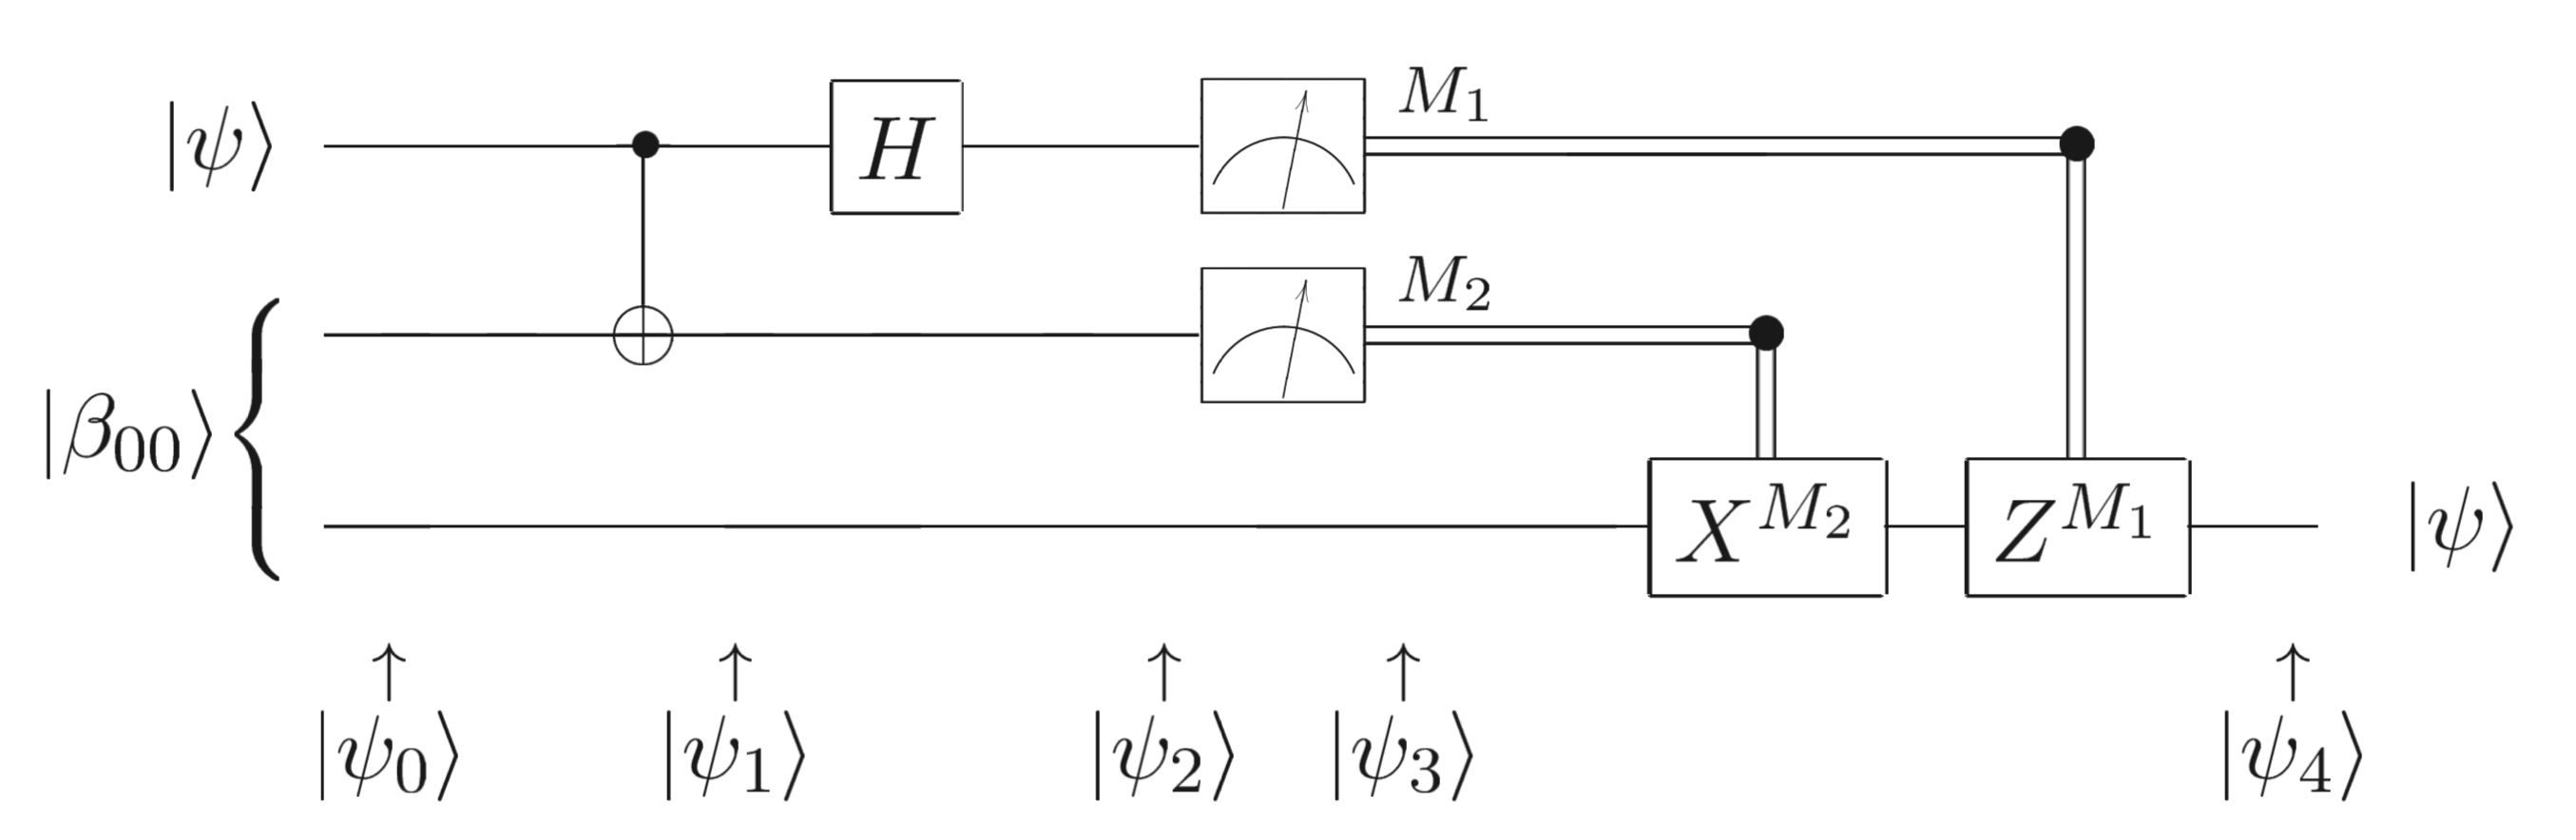
\includegraphics[width=\linewidth]{teleportation_circuit.png}	
\caption{Two top lines are Alice's system and bottom is Bob's}
\end{figure}

Recall the controlled-\texttt{NOT} (\texttt{CNOT}) takes $\ket{a}\ket{b}$ to $\ket{a}\ket{b \oplus a}$. The other gates in the circuit are summarized in the diagram below.

\begin{figure}[H]
\centering
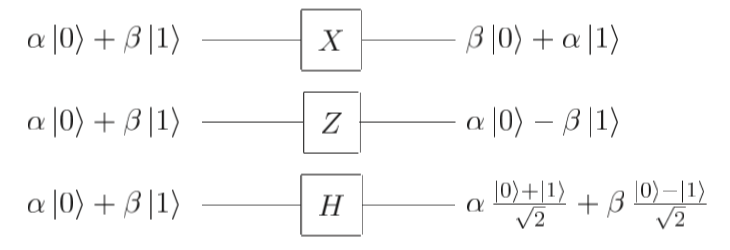
\includegraphics[width=0.5\linewidth]{basic_gates.png}	
\caption{Basic gates}
\end{figure}

So, the first two qubits belong to Alice and the third to Bob. Alice sends her qubits through a \texttt{CNOT} obtaining

\begin{align*}
\ket{\psi_1} &= \frac{1}{\sqrt{2}}\Big[\alpha\ket{0}(\ket{00} + \ket{11}) + \beta\ket{1}(\ket{10} + \ket{01})\Big]
\end{align*}

Then, Alice's first qubit is sent through a Hadamard gate which gives

\begin{align*}
\ket{\psi_2} &= \frac{1}{2}\Big[\alpha(\ket{0}+\ket{1})(\ket{00} + \ket{11}) + \beta(\ket{0}-\ket{1})(\ket{10} + \ket{01})\Big] \\
&= \frac{1}{2}\Big[ \ket{00} (\alpha\ket{0} + \beta\ket{1}) + \ket{01}(\alpha\ket{1} + \beta \ket{0}) + \ket{10}(\alpha\ket{0} - \beta\ket{1}) + \ket{11}(\alpha\ket{1} - \beta\ket{0}) \Big]
\end{align*}

Now, observe that each grouping in this expression has Alice's bits in a different state ($\ket{00},\ket{01},\ket{10},\ket{11}$), each of which Alice may observe after a measurement. Curiously, each of these groupings has a unique corresponding state for Bob's qubits. Hence, we know the state of Bob's qubits given knowledge of the outcome of Alice's measurement.

Furthermore, note that each of the possible states of Bob's qubits after Alice's measurements can be readily transformed to $\ket{\psi}$. Consider the four cases

\begin{enumerate}
\item Alice measures $00$. Hence, Bob's state is already $\ket{\psi}$. 
\item Alice measures $01$. Hence, Bob's state is $\alpha\ket{1} + \beta \ket{0}$. So, just apply the $X$ gate. 
\item Alice measures $10$. Hence, Bob's state is $\alpha\ket{0} - \beta\ket{1}$. So, just apply the $Z$ gate to flip the second sign. 
\item Alice measures $11$. Hence, Bob's state is $\alpha\ket{1} - \beta\ket{0}$. So, apply the $X$ gate to flip the bits, then the $Z$ gate to flip the second sign. 
\end{enumerate}

So that's what the notation in the circuit above means, we apply $X$ or $Z$ to Bob's qubits to recover $\ket{\psi}$ depending on the outcome of Alice's measurement.

Pretty cool, right? Let's look at this a level deeper using the density operator formalism we've developed. Each of the 4 cases have probability $\frac{1}{4}$ of occurring after the measurement. Hence, the density operator is given by

\begin{align*}
	\rho =& \frac{1}{4}\Big[ \ket{00}\bra{00} (\alpha\ket{0} + \beta\ket{1})(\alpha^*\bra{0} + \beta^*\bra{1}) + \ket{01}\bra{01}(\alpha\ket{1} + \beta \ket{0})(\alpha^*\bra{1} + \beta^* \bra{0}) \\
	&+ \ket{10}\bra{10}(\alpha\ket{0} - \beta\ket{1})(\alpha^*\bra{0} - \beta^*\bra{1}) + \ket{11}\bra{11}(\alpha\ket{1} - \beta\ket{0})(\alpha^*\bra{1} - \beta^*\bra{0}) \Big]
\end{align*}

So, the reduced density operator of Bob's system is

\begin{align*}
	\rho^B =& \frac{1}{4}\Big[ \bra{00}\ket{00} (\alpha\ket{0} + \beta\ket{1})(\alpha^*\bra{0} + \beta^*\bra{1}) + \bra{01}\ket{01}(\alpha\ket{1} + \beta \ket{0})(\alpha^*\bra{1} + \beta^* \bra{0}) \\
	&+ \bra{10}\ket{10}(\alpha\ket{0} - \beta\ket{1})(\alpha^*\bra{0} - \beta^*\bra{1}) + \bra{11}\ket{11}(\alpha\ket{1} - \beta\ket{0})(\alpha^*\bra{1} - \beta^*\bra{0}) \Big] \\
	=& \frac{1}{4}\Big[(\alpha\ket{0} + \beta\ket{1})(\alpha^*\bra{0} + \beta^*\bra{1}) + (\alpha\ket{1} + \beta \ket{0})(\alpha^*\bra{1} + \beta^* \bra{0}) \\
	&+ (\alpha\ket{0} - \beta\ket{1})(\alpha^*\bra{0} - \beta^*\bra{1}) + (\alpha\ket{1} - \beta\ket{0})(\alpha^*\bra{1} - \beta^*\bra{0}) \Big] \\
	=& \frac{1}{4}\Big[2(\alpha^*\alpha + \beta^*\beta)\ket{0}\bra{0} + 2(\alpha^*\alpha + \beta^*\beta)\ket{1}\bra{1}] \\
	=& \frac{I}{2}
\end{align*}
by $|\alpha|^2 + |\beta|^2 = 1$ and completeness.

Hence, the state of Bob's system after Alice has performed the measurement (but before Bob has learned the measurement result) is $I/2$ which has no dependence upon the state $\ket{\psi}$ being teleported. Therefore, any measurements performed by Bob will contain no information about $\ket{\psi}$, so information being communicated is dependent on the classical communication channel, implying that the speed of light limit is obeyed.

\subsection{The Schmidt Decomposition and purifications}

Schmidt Decomposition theorem says given a pure state $\ket{\psi}$ in a composite system $AB$, then there are orthonormal states $\ket{i_A}$ and $\ket{i_B}$ in $A$ and $B$, respectively, such that

\begin{align*}
\ket{\psi} = \sum_i \lambda_i \ket{i_A}\ket{i_B}	
\end{align*}

where $\lambda_i$ is nonnegative real and $\sum_i \lambda_i^2 = 1$.

One readily seen implication is that the spectra of $\rho^A$ and $\rho^B$ are the same, given a pure state in composite system $AB$. 

A second technique is purification. Suppose we are given a state $\rho^A$ of system $A$. We can then introduce another system $R$ and define a pure state $\ket{AR}$ for the joint system $AR$ such that $\rho^A = \tr_R (\ket{AR}\bra{AR})$. $R$ is simply a reference and has no physical significance, the point is that we can associate pure states with mixed states.
\subsection{EPR and the Bell Inequality}  

Imagine we perform the following measurement. Charlie prepares a quantum system of two qubits in the state

\begin{align*}
\ket{\psi} = \frac{\ket{01} - \ket{10}}{\sqrt{2}}	
\end{align*}

He passes the first bit to Alice and second to Bob. They perform measurements of the following observable

\begin{align*}
Q &= Z_1 \\
R &= X_1 \\
S &= \frac{-Z_2-X_2}{\sqrt{2}} \\
T &= \frac{Z_2 - X_2}{\sqrt{2}}	
\end{align*}

We can calculate and show that 

\begin{align*}
\langle QS \rangle &= \frac{1}{\sqrt{2}}\\	
\langle RS \rangle &= \frac{1}{\sqrt{2}}\\	
\langle RT \rangle &= \frac{1}{\sqrt{2}}\\	
\langle QT \rangle &= \frac{1}{\sqrt{2}}\\	
\end{align*}

\begin{proof}
% TODO fill in bell's calculations	
\end{proof}

and so $\langle QS \rangle + \langle RS \rangle + \langle RT \rangle - \langle QT \rangle = 2\sqrt{2}$. This violates Bell's inequality, derived in the text, which says that this value should never exceed 2. 

Bell's inequality requires assuming that $Q,R,S,T$ have definite values beforehand (realism). Additionally, we assumed that Alice performing the measurement does not influence the result of Bob's measurement (locality). Hence, at least one of these assumptions must be incorrect (since experimentation confirms this quantum picture).


\subsection{No-cloning Theorem}

It is impossible to copy an unknown quantum state.

\begin{proof}
Suppose we have a quantum machine with two slots labelled $A$ and $B$. Slot $A$ starts out with unknown state $\ket{\psi}$ which is two be copied to $B$. Assume that $B$ starts out with some pure state $\ket{s}$.

Hence, the initial state of the machine is $\ket{\psi}\ket{s}$. So, some unitary evolution $U$ now effects the copying procedure

\begin{align*}
	U(\ket{\psi}\ket{s}) = \ket{\psi}\ket{\psi}
\end{align*}
	
	Suppose this works for two particular states $\ket{\psi}$ and $\ket{\phi}$. Hence,
	
	\begin{align*}
		U(\ket{\psi}\ket{s}) = \ket{\psi}\ket{\psi} \\
		U(\ket{\phi}\ket{s}) = \ket{\phi}\ket{\phi}
	\end{align*}
	
	Hence, take the inner product of the two equations and 
	
	\begin{align*}
		(\bra{\phi}\ket{\psi}\bra{s}\ket{s})U^\dag U &= \bra{\phi}\ket{\psi} \\
		\bra{\psi}\ket{\phi}\bra{\psi}\ket{\phi} &= |\bra{\phi}\ket{\psi}|^2
	\end{align*}
	
	Hence, either $\bra{\phi}\ket{\psi}$ is 0 or 1. Thus, either $\ket{\psi} = \ket{\phi}$ (a contradiction to assuming they're distinct) or the two states are orthogonal.
	
	Therefore, a cloning device can only clone states which are orthogonal to one another and so a general quantum cloning device is impossible.  
\end{proof}

\section{Nielsen \& Chuang: Chapter 4}

\section{Nielsen \& Chuang: Chapter 5}

\begin{enumerate}
\item Quantum Fourier Transform
\item Quantum Phase Estimation Algorithm
\item Shor's algorithm for Factoring
\end{enumerate}

\section{Nielsen \& Chuang: Chapter 6}

Quantum Search algorithms

\section{Algorithms for solving linear systems of equations}
\url{https://arxiv.org/abs/0811.3171}

\section{Density Matrix Exponentiation Algorithms}
\url{https://www.nature.com/articles/nphys3029}

\section{Review of Quantum Machine Learning}
\url{https://www.nature.com/articles/nature23474}

\section{Learnability of Quantum States}
\begin{enumerate}
\item \url{https://arxiv.org/abs/quant-ph/0608142}
\item \url{https://arxiv.org/abs/1711.01053}
\item \url{https://arxiv.org/abs/1801.05721}
\end{enumerate}


\section{Appendix}

\subsection{Pauli Matrices}\label{pauli}
\begin{align*}
\sigma_x &= X = \begin{pmatrix} 0 & 1 \\ 1 & 0\end{pmatrix} \\
\sigma_y &= Y = \begin{pmatrix} 0 & -i \\ i & 0\end{pmatrix}\\
\sigma_z &= Z = \begin{pmatrix} 1 & 0 \\ 0 & -1\end{pmatrix}
\end{align*}

\subsection{Bell States}\label{bellstates}
\begin{align*}
\frac{\ket{00} + \ket{11} }{\sqrt{2}} \\	
\frac{\ket{00} - \ket{11} }{\sqrt{2}} \\	
\frac{\ket{10} + \ket{01} }{\sqrt{2}} \\	
\frac{\ket{01} - \ket{10} }{\sqrt{2}}
\end{align*}

\subsection{Positive Operators}\label{posop}
Let $A$ be a bounded\footnote{$\Vert Av \Vert \leq M\Vert v \Vert$ for some $M>0$ and all $v \in \mathcal{H}$} linear operator on complex Hilbert space $\mathcal{H}$. The following conditions are equivalent to $A$ being positive

\begin{enumerate}
\item $A=S^\dag S$ for some bounded operator $S$ on $\mathcal{H}$
\item $A$ is hermitian and $\bra{x} A \ket{x} \geq 0$ for every $\ket{x} \in \mathcal{H}$
\item the spectrum of $A$ is non-negative
\end{enumerate}

\subsection{Trace of an Operator}\label{trop}

Let $\{\ket{i}\}$ be an orthonormal basis for $A$ and so
\begin{align*}
\tr(A) &= \sum_i A_{ii} \\
&= \sum_i \bra{i} A \ket{i}	
\end{align*}

Hence, if we extend $\ket{\psi}$ to the orthonormal basis $\{\ket{i}\}$ which includes $\ket{\psi}$ as the first element (for example via the Gram-Schmidt procedure) then

\begin{align*}
	\tr(A\ket{\psi}\bra{\psi}) &= \sum_i \bra{i} A\ket{\psi}\bra{\psi}\ket{i}	 \\
	&= \bra{\psi} A\ket{\psi}
\end{align*}

by orthonormality.

\subsection{Spectral Theorem}
Suppose $A$ is a compact\footnote{the image under $A$ acting on any bounded subset of $\mathcal{H}$ is a compact subset of $\mathcal{H}$} hermitian operator (compactness ensures $A$ has eigenvectors) on complex Hilbert space $\mathcal{H}$. Hence, there is an orthonormal basis of $\mathcal{H}$ consisting of eigenvectors of $A$. Each eigenvalue is in $\RR$.

\nocite{*}
\bibliographystyle{plain}
\bibliography{course_notes}

\end{document}
